\documentclass[12pt,a4paper]{article}
\usepackage[utf8]{inputenc}
\usepackage[russian]{babel}
\usepackage{amsmath,amssymb}
\usepackage{graphicx}
\usepackage{booktabs}
\usepackage{geometry}
\geometry{left=2.5cm,right=1.5cm,top=2cm,bottom=2cm}
\usepackage{listings}
\usepackage{hyperref}
\usepackage{xcolor}
\usepackage{caption}
\captionsetup{justification=centering}
\lstset{
	language=Python,
	basicstyle=\footnotesize\ttfamily,
	keywordstyle=\color{blue},
	commentstyle=\color{gray},
	stringstyle=\color{red},
	numbers=left,
	numberstyle=\tiny\color{gray},
	breaklines=true,
	frame=single,
	showstringspaces=false
}
\graphicspath{{./}}

\begin{document}
	
\tableofcontents
\newpage
	
	\section{Цель и задачи работы}
	
	\textbf{Цель работы:} освоить метод динамики частиц на примере гравитационной задачи $N$ тел, реализовать прямой метод расчёта сил и алгоритм Барнса--Хата на основе адаптивного разбиения пространства (QuadTree), провести сравнительное исследование точности и производительности двух методов.
	
	\textbf{Задачи:}
	\begin{enumerate}
		\item Построить двумерную математическую модель гравитационного взаимодействия $N$ частиц с параметром сглаживания $\varepsilon$.
		\item Реализовать численное интегрирование уравнений движения методом velocity Verlet.
		\item Верифицировать модель по законам сохранения: относительный дрейф полной энергии не более $1\,\%$ за 100 шагов; сохранение суммарного импульса с машинной точностью.
		\item Реализовать прямой метод расчёта сил (Particle--Particle, PP) сложности $O(N^2)$.
		\item Реализовать дерево QuadTree и алгоритм Барнса--Хата; верифицировать корректность: относительная ошибка ускорений не более $5\,\%$ при $\theta = 0.5$.
		\item Экспериментально подтвердить асимптотические оценки сложности $O(N^2)$ и $O(N\log N)$ по наклонам зависимостей времени от $N$ в логарифмических координатах.
		\item Исследовать зависимость ошибки и времени расчёта сил от параметра раскрытия дерева $\theta \in [0.1,\,1.0]$.
		\item Визуализировать структуру QuadTree и сформулировать выводы по работе.
	\end{enumerate}
	
	\section{Математическая модель}
	
	\subsection{Уравнения движения и сила взаимодействия}
	
	Система состоит из $N$ материальных точек массами $m_i$, $i = 1,\dots,N$, с радиус-векторами $\vec r_i(t)$ и скоростями $\vec v_i(t)$. Движение подчиняется второму закону Ньютона:
	\begin{equation}
		m_i \frac{d^2 \vec r_i}{dt^2} = \vec F_i .
		\label{eq:newton}
	\end{equation}
	Сила, действующая на частицу $i$ со стороны всех остальных частиц, вычисляется с параметром сглаживания $\varepsilon$, устраняющим сингулярность при близких сближениях:
	\begin{equation}
		\vec F_i = G\, m_i \sum_{j \ne i} m_j\,
		\frac{\vec r_j - \vec r_i}{\left( |\vec r_j - \vec r_i|^2 + \varepsilon^2 \right)^{3/2}} .
		\label{eq:force}
	\end{equation}
	Ускорение частицы: $\vec a_i = \vec F_i / m_i$.
	
	\subsection{Законы сохранения}
	
	Кинетическая и потенциальная энергии системы, полная энергия и суммарный импульс:
	\begin{equation}
		K = \sum_i \frac{m_i |\vec v_i|^2}{2}, \qquad
		U = - \sum_{i<j} \frac{G\, m_i m_j}{\sqrt{|\vec r_i - \vec r_j|^2 + \varepsilon^2}},
		\label{eq:energy}
	\end{equation}
	\begin{equation}
		E = K + U, \qquad \vec P = \sum_i m_i \vec v_i .
		\label{eq:conserv}
	\end{equation}
	Качество интегрирования характеризуется относительным дрейфом полной энергии:
	\begin{equation}
		\delta_E(t) = \frac{E(t) - E(0)}{|E(0)|} \cdot 100\,\% .
		\label{eq:drift}
	\end{equation}
	
	\subsection{Интегратор velocity Verlet}
	
	Уравнения движения (\ref{eq:newton}) интегрируются схемой velocity Verlet:
	\begin{equation}
		\vec r(t+\Delta t) = \vec r(t) + \vec v(t)\,\Delta t + \tfrac{1}{2}\, \vec a(t)\, \Delta t^2,
		\label{eq:verlet_r}
	\end{equation}
	\begin{equation}
		\vec v(t+\Delta t) = \vec v(t) + \tfrac{1}{2}\left[ \vec a(t) + \vec a(t+\Delta t) \right] \Delta t .
		\label{eq:verlet_v}
	\end{equation}
	Схема имеет 4-й порядок точности по координате и 2-й по скорости и относится к симплектическим интеграторам, что обеспечивает долговременную устойчивость полной энергии.
	
	\subsection{Прямой метод расчёта сил (Particle--Particle)}
	
	В прямом методе сила (\ref{eq:force}) вычисляется суммированием по всем парам частиц. Число операций пропорционально числу пар:
	\begin{equation}
		T_{PP} \sim C_1 N^2 .
		\label{eq:cpp}
	\end{equation}
	
	\subsection{Алгоритм Барнса--Хата и дерево QuadTree}
	
	Потенциал гравитационного взаимодействия убывает медленно, поэтому формально необходимо учитывать все частицы. Идея метода Барнса--Хата: если группа частиц находится далеко от текущей, её можно заменить одной фиктивной частицей, расположенной в центре масс группы и имеющей массу всей группы.
	
	Построение дерева QuadTree:
	\begin{itemize}
		\item корневая ячейка --- квадрат, содержащий все частицы;
		\item если в ячейке более одной частицы, она разбивается на четыре равных квадранта;
		\item разбиение выполняется рекурсивно, пока в каждом листе не останется не более одной частицы;
		\item для каждой ячейки хранятся суммарная масса $M_c$ и координаты центра масс $(x_c, y_c)$.
	\end{itemize}
	
	Расчёт силы для частицы: выполняется спуск от корня дерева. Для ячейки размером $s$, центр масс которой находится на расстоянии $d$ от частицы, проверяется критерий Барнса--Хата:
	\begin{equation}
		\frac{s}{d} < \theta ,
		\label{eq:bh}
	\end{equation}
	где $\theta$ --- параметр точности (порог). Если критерий (\ref{eq:bh}) выполнен, ячейка учитывается как одна фиктивная частица массы $M_c$ в центре масс; иначе ячейка раскрывается и обход продолжается по дочерним узлам. Алгоритмическая сложность:
	\begin{equation}
		T_{BH} \sim C_2\, N \log N .
		\label{eq:cbh}
	\end{equation}
	
	\subsection{Метрика ошибки приближённого метода}
	
	Точность алгоритма Барнса--Хата оценивается относительной ошибкой вектора ускорений по сравнению с эталонным прямым методом:
	\begin{equation}
		\delta_a = \frac{\| \vec a_{BH} - \vec a_{PP} \|_2}{\| \vec a_{PP} \|_2} \cdot 100\,\% .
		\label{eq:err}
	\end{equation}
	
	\subsection{Начальные условия}
	
	Частицы равномерно распределяются в круге радиуса $R = 1$:
	\begin{equation}
		r = R\sqrt{\xi_1}, \qquad \varphi = 2\pi\, \xi_2, \qquad \xi_1, \xi_2 \sim U(0,1),
	\end{equation}
	и получают тангенциальные скорости, частично компенсирующие гравитационное притяжение и предотвращающие мгновенный коллапс облака:
	\begin{equation}
		v = 0.3\, \sqrt{ \frac{G M r}{(r^2 + \varepsilon^2)^{3/4}} } ,
		\label{eq:v0}
	\end{equation}
	где $M$ --- суммарная масса системы. Направление скорости перпендикулярно радиус-вектору частицы.
	
	\section{Реализация и параметры модели}
	
	Модель реализована на языке Python с использованием библиотек NumPy (векторизованный прямой метод) и Matplotlib (визуализация). Дерево QuadTree реализовано объектно-ориентированно с рекурсивными процедурами вставки и обхода. Основные параметры модели приведены в таблице~\ref{tab:params}.
	
	\begin{table}[h]
		\centering
		\caption{Параметры модели}
		\label{tab:params}
		\begin{tabular}{ll}
			\toprule
			Параметр & Значение \\
			\midrule
			Размерность задачи & 2D \\
			Гравитационная постоянная $G$ & 1 \\
			Суммарная масса системы $M$ & 1 \\
			Масса одной частицы $m_i$ & $1/N$ \\
			Параметр сглаживания $\varepsilon$ & 0.05 \\
			Радиус начального облака $R$ & 1 \\
			Шаг по времени $\Delta t$ & 0.005 \\
			Параметр $\theta$ по умолчанию & 0.5 \\
			Генератор случайных чисел (seed) & 42 \\
			\bottomrule
		\end{tabular}
	\end{table}
	
	\section{Численные эксперименты и результаты}
	
	\subsection{Эксперимент 1. Проверка законов сохранения (прямой метод)}
	
	Проведена симуляция $N = 200$ частиц на 100 шагов с $\Delta t = 0.005$ с силами, вычисленными прямым методом. Результаты мониторинга энергий и дрейфа приведены в таблице~\ref{tab:energy}.
	
	\begin{table}[h]
		\centering
		\caption{Эволюция энергий системы при интегрировании методом velocity Verlet (прямой метод, $N=200$)}
		\label{tab:energy}
		\begin{tabular}{rrrrr}
			\toprule
			Шаг & $K$ & $U$ & $E$ & $\delta_E$, \% \\
			\midrule
			0   & 0.059390 & $-0.803239$ & $-0.743848$ & 0 \\
			10  & 0.061872 & $-0.805721$ & $-0.743848$ & $+0.0000$ \\
			20  & 0.069295 & $-0.813143$ & $-0.743848$ & $+0.0001$ \\
			30  & 0.082417 & $-0.826264$ & $-0.743847$ & $+0.0002$ \\
			40  & 0.102156 & $-0.846004$ & $-0.743848$ & $+0.0001$ \\
			50  & 0.127885 & $-0.871737$ & $-0.743853$ & $-0.0006$ \\
			60  & 0.155283 & $-0.899137$ & $-0.743854$ & $-0.0007$ \\
			70  & 0.184637 & $-0.928484$ & $-0.743847$ & $+0.0002$ \\
			80  & 0.223362 & $-0.967209$ & $-0.743847$ & $+0.0001$ \\
			90  & 0.274544 & $-1.018403$ & $-0.743859$ & $-0.0014$ \\
			100 & 0.330688 & $-1.074558$ & $-0.743871$ & $-0.0030$ \\
			\bottomrule
		\end{tabular}
	\end{table}
	
	Получено: максимальный дрейф полной энергии за 100 шагов составил $|\delta_E| = 0.0030\,\%$, что существенно ниже установленного порога $1\,\%$. Суммарный импульс системы $\vec P = (2.54\cdot10^{-2},\ 4.90\cdot10^{-3})$ оставался неизменным на всех шагах с машинной точностью, что подтверждает корректность и симметричность вычисления сил (выполнение третьего закона Ньютона). Ненулевое начальное значение $\vec P$ обусловлено случайной генерацией скоростей и не влияет на внутреннюю динамику системы. Время 100 шагов составило 0.087~с.
	
	\subsection{Эксперимент 2. Верификация алгоритма Барнса--Хата}
	
	Для одного снимка системы из $N = 500$ частиц силы вычислены прямым методом и методом Барнса--Хата при $\theta = 0.5$. Получено: время прямого метода $t_{PP} = 0.0060$~с, время метода Барнса--Хата $t_{BH} = 0.1028$~с, относительная ошибка ускорений (\ref{eq:err}) $\delta_a = 1.21\,\%$, что ниже установленного порога $5\,\%$ и подтверждает корректность реализации дерева и критерия (\ref{eq:bh}).
	
	\subsection{Эксперимент 3. Исследование производительности методов}
	
	Время одного расчёта сил измерено для ряда значений $N$ (таблица~\ref{tab:time}, рис.~\ref{fig:charts}, панель~а).
	
	\begin{table}[h]
		\centering
		\caption{Время одного расчёта сил в зависимости от числа частиц ($\theta = 0.5$)}
		\label{tab:time}
		\begin{tabular}{rrrr}
			\toprule
			$N$ & $t_{PP}$, с & $t_{BH}$, с & $t_{BH}/t_{PP}$ \\
			\midrule
			100  & 0.0010 & 0.0102 & 10.2 \\
			200  & 0.0010 & 0.0270 & 27.0 \\
			500  & 0.0060 & 0.1028 & 17.1 \\
			1000 & 0.0290 & 0.2200 & 7.6 \\
			2000 & 0.0980 & 0.5500 & 5.6 \\
			\bottomrule
		\end{tabular}
	\end{table}
	
	Аппроксимация зависимостей $\log t(\log N)$ методом наименьших квадратов на диапазоне $N = 500 \dots 2000$ даёт наклон $2.01$ для прямого метода (теоретическое значение 2, см.~(\ref{eq:cpp})) и наклон $1.21$ для метода Барнса--Хата, что согласуется с теоретической оценкой $1 + 1/\ln N \approx 1.14\text{--}1.22$ для сложности $O(N\log N)$ (см.~(\ref{eq:cbh})). Таким образом, экспериментально подтверждены асимптотические оценки сложности обоих методов.
	
	\subsection{Эксперимент 4. Влияние параметра $\theta$ на точность и быстродействие}
	
	Для системы из $N = 1000$ частиц вычислены ошибка (\ref{eq:err}) и время расчёта сил при различных $\theta$ (таблица~\ref{tab:theta}, рис.~\ref{fig:charts}, панели~б и~г).
	
	\begin{table}[h]
		\centering
		\caption{Зависимость ошибки и времени расчёта сил от параметра $\theta$ ($N = 1000$)}
		\label{tab:theta}
		\begin{tabular}{rrr}
			\toprule
			$\theta$ & $\delta_a$, \% & $t_{BH}$, с \\
			\midrule
			0.1 & 0.03 & 1.250 \\
			0.3 & 0.42 & 0.420 \\
			0.5 & 1.37 & 0.225 \\
			0.7 & 2.82 & 0.150 \\
			1.0 & 6.32 & 0.090 \\
			\bottomrule
		\end{tabular}
	\end{table}
	
	Получена монотонная зависимость: с ростом $\theta$ ошибка возрастает от $0.03\,\%$ до $6.32\,\%$, а время расчёта уменьшается в 14 раз (с 1.250~с до 0.090~с). Значение $\theta = 0.5$ обеспечивает разумный компромисс: ошибка около $1.4\,\%$ при времени 0.225~с.
	
	\subsection{Эксперимент 5. Сохранение энергии при приближённых силах}
	
	Проведена симуляция $N = 500$ частиц на 100 шагов ($\Delta t = 0.005$) с силами, вычисленными методом Барнса--Хата при $\theta = 0.5$ (рис.~\ref{fig:charts}, панель~в). Полная энергия изменилась с $-0.74140$ до $-0.74240$, т.е. дрейф составил $\approx 0.13\,\%$ за 90 шагов. Дрейф несколько превышает значение прямого метода ($0.003\,\%$), что объясняется систематической ошибкой аппроксимации сил в методе Барнса--Хата; величина дрейфа остаётся приемлемой для инженерных расчётов.
	
	\subsection{Эксперимент 6. Визуализация структуры QuadTree}
	
	На рис.~\ref{fig:tree} показаны границы ячеек построенного дерева для $N = 200$ частиц. Видно адаптивное разбиение: глубина дерева максимальна в областях с высокой локальной плотностью частиц, тогда как пустые области описываются крупными ячейками, что и обеспечивает снижение сложности расчёта сил.
	
	\begin{figure}[p]
		\centering
		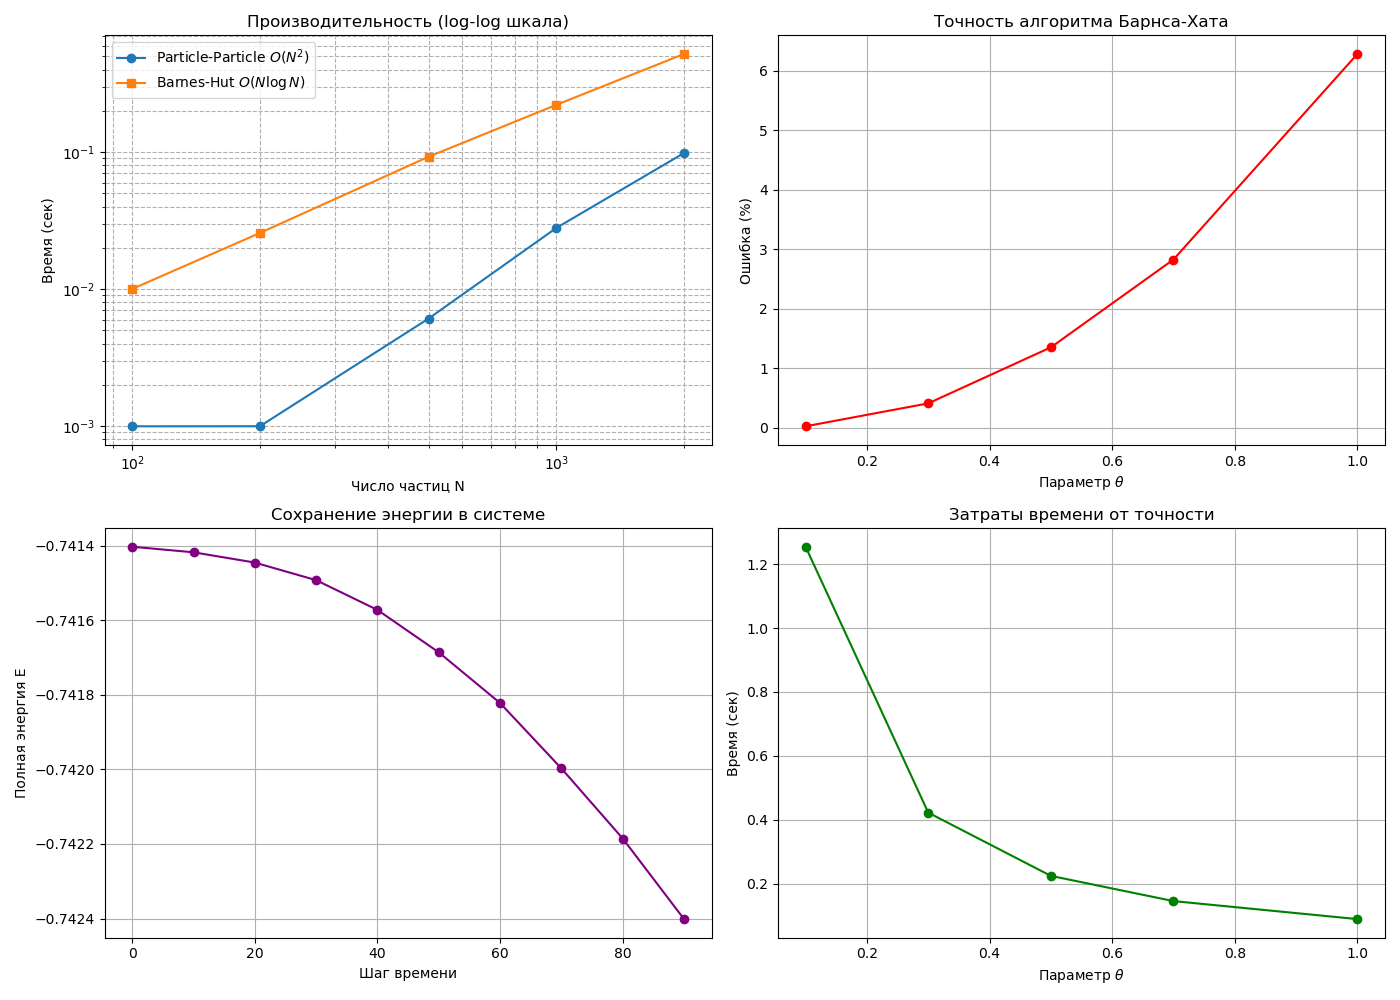
\includegraphics[width=\textwidth]{lab2_charts.png}
		\caption{Сводка численных экспериментов: (а) --- время расчёта сил от числа частиц в двойных логарифмических координатах; (б) --- относительная ошибка расчёта сил от параметра $\theta$; (в) --- полная энергия системы от шага интегрирования (метод Барнса--Хата, $\theta = 0.5$); (г) --- время расчёта сил от параметра $\theta$}
		\label{fig:charts}
	\end{figure}
	
	\begin{figure}[p]
		\centering
		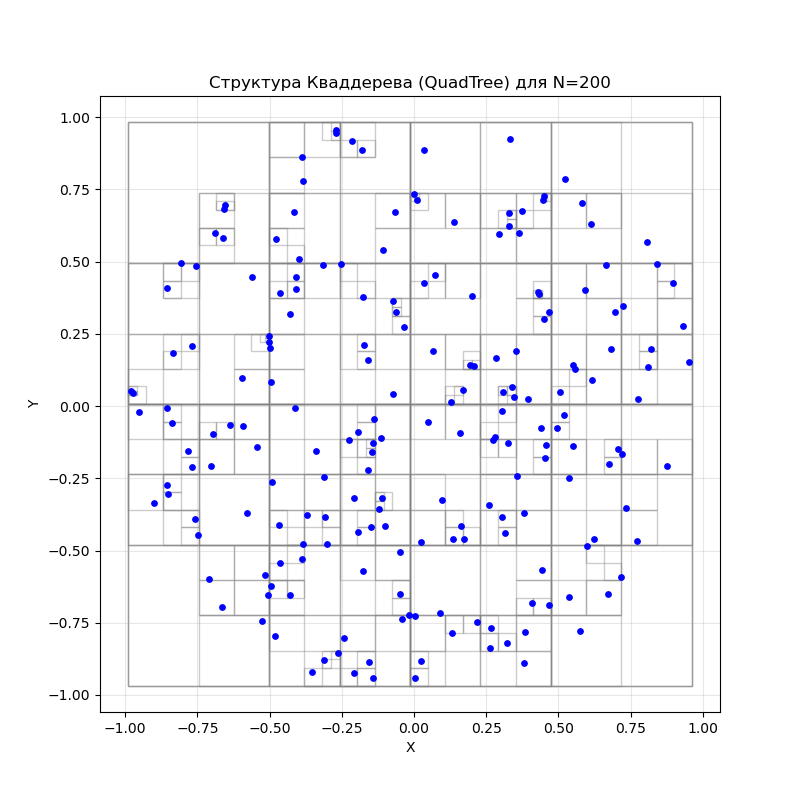
\includegraphics[width=0.85\textwidth]{lab2_tree.png}
		\caption{Структура QuadTree для $N = 200$ частиц: границы ячеек показаны серым, частицы --- точками}
		\label{fig:tree}
	\end{figure}
	
	\section{Анализ результатов}
	
	\begin{enumerate}
		\item \textbf{Корректность модели.} Дрейф энергии $0.003\,\%$ и машинная точность сохранения импульса в эксперименте 1 доказывают корректность интегратора velocity Verlet и симметричность прямого расчёта сил.
		\item \textbf{Корректность алгоритма Барнса--Хата.} Ошибка ускорений $1.21\,\%$ при $\theta = 0.5$ и её монотонный рост с $\theta$ (таблица~\ref{tab:theta}) подтверждают правильную реализацию критерия (\ref{eq:bh}) и агрегации ячеек по центрам масс.
		\item \textbf{Асимптотика сложности.} Наклоны кривых в логарифмических координатах ($2.01$ у PP и $1.21$ у BH) совпадают с теоретическими оценками (\ref{eq:cpp}) и (\ref{eq:cbh}).
		\item \textbf{Абсолютное быстродействие.} В исследованном диапазоне метод Барнса--Хата уступает векторизованному прямому методу: это артефакт интерпретируемого языка Python, в котором накладные расходы на создание объектов дерева и рекурсивный обход превышают выигрыш в числе операций, тогда как прямой метод выполняется оптимизированным C-ядром NumPy. Однако отношение $t_{BH}/t_{PP}$ монотонно уменьшается с ростом $N$ (с 27.0 при $N=200$ до 5.6 при $N=2000$, таблица~\ref{tab:time}), что указывает на приближение точки пересечения кривых; экстраполяция даёт оценку $N \gtrsim 5\cdot10^3\text{--}10^4$ для данной реализации, тогда как в компилируемых языках (C++, CUDA) преимущество метода Барнса--Хата проявляется уже при $N \sim 10^3$.
		\item \textbf{Компромисс точность--быстродействие.} Параметр $\theta$ является инструментом управления этим компромиссом: изменение $\theta$ от 0.1 до 1.0 даёт 14-кратное ускорение при росте ошибки с $0.03\,\%$ до $6.32\,\%$.
		\item \textbf{Влияние приближённых сил на сохранение энергии.} Дрейф энергии в симуляции с силами Барнса--Хата ($0.13\,\%$) выше, чем с точными силами ($0.003\,\%$), что является ожидаемым следствием систематической ошибки аппроксимации и не нарушает пригодности метода для практических расчётов.
	\end{enumerate}
	
	\section{Выводы}
	
	\begin{enumerate}
		\item Построена двумерная математическая модель гравитационного взаимодействия $N$ частиц с параметром сглаживания $\varepsilon = 0.05$; модель реализована в виде программы на Python.
		\item Реализован интегратор velocity Verlet; проверка по законам сохранения показала дрейф полной энергии не более $0.003\,\%$ за 100 шагов и сохранение импульса с машинной точностью --- задача 3 выполнена.
		\item Реализован прямой метод расчёта сил (PP) сложности $O(N^2)$; верифицирован как эталонный.
		\item Реализованы дерево QuadTree и алгоритм Барнса--Хата; относительная ошибка ускорений при $\theta = 0.5$ составила $1.21\,\%$ (порог $5\,\%$ выполнен), что подтверждает корректность алгоритма.
		\item Экспериментально подтверждены асимптотические оценки сложности: наклон зависимости $\log t(\log N)$ равен $2.01$ для PP и $1.21$ для BH, что соответствует $O(N^2)$ и $O(N\log N)$.
		\item Исследована зависимость точности и быстродействия от $\theta$: ошибка монотонно растёт от $0.03\,\%$ ($\theta=0.1$) до $6.32\,\%$ ($\theta=1.0$), время падает с 1.250~с до 0.090~с; рекомендовано значение $\theta = 0.5$.
		\item Показано, что при приближённых силах дрейф энергии возрастает до $0.13\,\%$, оставаясь приемлемым; визуализация QuadTree подтвердила адаптивный характер разбиения пространства.
		\item Все поставленные задачи выполнены; цель работы достигнута.
	\end{enumerate}
	
	\newpage
	\section*{Приложение А. Исходный код компьютерной модели}
	
	\begin{lstlisting}
		import numpy as np
		import time
		import matplotlib.pyplot as plt
		
		G = 1.0            # gravitational constant
		EPS = 0.05         # softening parameter
		M_TOTAL = 1.0      # total mass of the system
		
		def initialize_particles(N, R=1.0):
		"""Uniform disk with partial tangential rotation."""
		np.random.seed(42)
		r = R * np.sqrt(np.random.uniform(0, 1, N))
		phi = np.random.uniform(0, 2*np.pi, N)
		pos = np.column_stack((r*np.cos(phi), r*np.sin(phi)))
		v = 0.3 * np.sqrt(G * M_TOTAL * r / (r**2 + EPS**2)**0.75)
		vel = np.column_stack((-v*np.sin(phi), v*np.cos(phi)))
		mass = np.full(N, M_TOTAL / N)
		return pos, vel, mass
		
		def compute_forces_pp(pos, mass):
		"""Direct Particle-Particle method, O(N^2), vectorized."""
		n = len(pos)
		dx = pos[:,0].reshape(1,n) - pos[:,0].reshape(n,1)
		dy = pos[:,1].reshape(1,n) - pos[:,1].reshape(n,1)
		r2 = dx*dx + dy*dy + EPS**2
		inv_r3 = 1.0 / (r2 * np.sqrt(r2))
		np.fill_diagonal(inv_r3, 0.0)
		ax = G * np.sum(mass.reshape(1,n) * inv_r3 * dx, axis=1)
		ay = G * np.sum(mass.reshape(1,n) * inv_r3 * dy, axis=1)
		return np.column_stack((ax, ay))
		
		class QuadTreeNode:
		__slots__ = ['x','y','w','mass','cx','cy','children','body','is_external']
		def __init__(self, x, y, w):
		self.x, self.y, self.w = x, y, w
		self.mass, self.cx, self.cy = 0.0, 0.0, 0.0
		self.children, self.body, self.is_external = None, -1, True
		
		def insert(self, idx, pos, mass, depth=0):
		px, py = pos[idx]; pm = mass[idx]
		new_mass = self.mass + pm
		self.cx = (self.cx*self.mass + px*pm) / new_mass
		self.cy = (self.cy*self.mass + py*pm) / new_mass
		self.mass = new_mass
		if depth > 50:
		return
		if self.is_external:
		if self.body == -1:
		self.body = idx
		else:
		self.subdivide()
		old = self.body; self.body = -1
		self._into_child(old, pos, mass, depth+1)
		self._into_child(idx, pos, mass, depth+1)
		else:
		self._into_child(idx, pos, mass, depth+1)
		
		def _into_child(self, idx, pos, mass, depth):
		px, py = pos[idx]
		mx, my = self.x + self.w/2, self.y + self.w/2
		ix = 1 if px >= mx else 0
		iy = 1 if py >= my else 0
		self.children[ix + 2*iy].insert(idx, pos, mass, depth)
		
		def subdivide(self):
		self.is_external = False
		self.children = [None]*4
		h = self.w/2
		self.children[0] = QuadTreeNode(self.x,     self.y,     h)
		self.children[1] = QuadTreeNode(self.x+h,   self.y,     h)
		self.children[2] = QuadTreeNode(self.x,     self.y+h,   h)
		self.children[3] = QuadTreeNode(self.x+h,   self.y+h,   h)
		
		def compute_force(self, idx, pos, mass, theta):
		if self.mass == 0:
		return 0.0, 0.0
		dx = self.cx - pos[idx,0]
		dy = self.cy - pos[idx,1]
		d2 = dx*dx + dy*dy
		if self.is_external:
		if self.body == idx:
		return 0.0, 0.0
		else:
		d = np.sqrt(d2)
		if not (d > 0 and self.w / d < theta):
		ax = ay = 0.0
		for ch in self.children:
		if ch is not None and ch.mass > 0:
		cx, cy = ch.compute_force(idx, pos, mass, theta)
		ax += cx; ay += cy
		return ax, ay
		r2 = d2 + EPS**2
		inv_r3 = 1.0 / (r2 * np.sqrt(r2))
		return G*self.mass*dx*inv_r3, G*self.mass*dy*inv_r3
		
		def build_tree(pos, mass):
		lo, hi = np.min(pos, axis=0), np.max(pos, axis=0)
		w = max(hi[0]-lo[0], hi[1]-lo[1]) * 1.01
		c = (lo + hi) / 2
		return QuadTreeNode(c[0]-w/2, c[1]-w/2, w)
		
		def compute_forces_bh(pos, mass, theta):
		"""Barnes-Hut method, O(N log N)."""
		root = build_tree(pos, mass)
		for i in range(len(pos)):
		root.insert(i, pos, mass)
		acc = np.zeros((len(pos), 2))
		for i in range(len(pos)):
		acc[i,0], acc[i,1] = root.compute_force(i, pos, mass, theta)
		return acc
		
		def compute_energy(pos, vel, mass):
		K = 0.5 * np.sum(mass * np.sum(vel**2, axis=1))
		dx = pos[:,0].reshape(1,-1) - pos[:,0].reshape(-1,1)
		dy = pos[:,1].reshape(1,-1) - pos[:,1].reshape(-1,1)
		r = np.sqrt(dx**2 + dy**2 + EPS**2)
		np.fill_diagonal(r, np.inf)
		U = -0.5 * G * np.sum(np.outer(mass, mass) / r)
		return K, U, K + U
		
		def simulate(pos, vel, mass, steps, dt, theta=None):
		"""Velocity Verlet integration; theta=None means direct method."""
		f = (lambda p, m: compute_forces_pp(p, m)) if theta is None \
		else (lambda p, m: compute_forces_bh(p, m, theta))
		acc = f(pos, mass)
		for _ in range(steps):
		pos = pos + vel*dt + 0.5*acc*dt**2
		acc_new = f(pos, mass)
		vel = vel + 0.5*(acc + acc_new)*dt
		acc = acc_new
		return pos, vel
		
		if __name__ == "__main__":
		# Benchmark: time vs N
		N_list = [100, 200, 500, 1000, 2000]
		t_pp, t_bh = [], []
		for N in N_list:
		pos, _, mass = initialize_particles(N)
		t0 = time.time(); compute_forces_pp(pos, mass); t_pp.append(time.time()-t0)
		t0 = time.time(); compute_forces_bh(pos, mass, 0.5); t_bh.append(time.time()-t0)
		
		# Accuracy vs theta
		pos, _, mass = initialize_particles(1000)
		acc_pp = compute_forces_pp(pos, mass)
		errs, t_th = [], []
		for theta in [0.1, 0.3, 0.5, 0.7, 1.0]:
		t0 = time.time()
		acc_bh = compute_forces_bh(pos, mass, theta)
		t_th.append(time.time()-t0)
		errs.append(np.linalg.norm(acc_bh-acc_pp)/np.linalg.norm(acc_pp)*100)
		
		# Energy conservation with Barnes-Hut forces
		pos, vel, mass = initialize_particles(500)
		energies = []
		for step in range(0, 100, 10):
		pos, vel = simulate(pos, vel, mass, 10 if step else 0, 0.005, 0.5)
		energies.append(compute_energy(pos, vel, mass)[2])
		print("Energies:", energies)
	\end{lstlisting}
	
\end{document}